% ==================================================================
\section{Recursive: Leaf Task Decomposition}
\label{sec:rec-leaf}
% ==================================================================

\subsection{Implementation}
\label{sec:rec-leaf-impl}
El codi de la versió \textbf{leaf recursive} es troba a \texttt{mandel-omp-leaf.c}.\\
El primer que analitzarem és que la regió paral·lela es crea al main, abans de la crida a \texttt{mandel\_tiled\_rec}, declarant la regió com a \texttt{single}. Això provocarà que un únic thread crei les tasques i faci el recorregut recursiu (és com funciona l'estratègia \textbf{leaf}).

\begin{lstlisting}[caption={Regió paral·lela i crida inicial al \texttt{main}.},label={lst:rec-leaf-main}]
#pragma omp parallel
#pragma omp single
mandel_tiled_rec((int (*)[width])Hmatrix, height, width, 0, 0,
             real_min, imag_min, real_max, imag_max,
             scale_real, scale_imag, maxiter);
\end{lstlisting}

Posteriorment, veiem que només es creen tasques a les fulles de l'arbre de recursió, en dos casos. O bé quan \texttt{equal} és cert, és a dir, les boreres del tile són iguals i es pot omplir el tile amb un valor uniforme, o bé quan el nombre de columnes és menor o igual que la mida del tile, cosa que indica que s'ha arribat a un tile prou petit perquè es calculi directament. En ambdós casos es crea una tasca per dur a terme l'operació corresponent. Vegeu-ho al propi codi, no s'adjunta perquè cada cas base ocupa moltes línies.\\
Si no es compleix cap de les condicions anteriors, la recursió es fa als quatre quadrants del tile (o a les dues meitats de columnes), però sense crear tasques per a aquestes crides recursives, cosa característica de l'estratègia \textbf{leaf}.\\
Cal destacar també que s'han evitat els problemes de compartició de dades en els accessos a l'histograma i a la biblioteca X detectats a la pràctica 3, de la manera següent:
\begin{itemize}
    \item Per l'accès a histograma, s'ha utilitzat \texttt{\#pragma omp atomic}:
    \begin{lstlisting}[language=C]
#pragma omp atomic
histogram[M[y][x] - 1] += (NRows * NCols);
    \end{lstlisting}

    \item Per l'accès a la librería X, las instruccions s'han protegit amb \texttt{\#pragma omp critical}:
    \begin{lstlisting}[language=C]
#pragma omp critical
{
    XSetForeground(display, gc, color);
    XDrawPoint(display, win, gc, px, py);
}
    \end{lstlisting}
\end{itemize}

\subsection{Modelfactor Analysis}
\label{sec:rec-leaf-mf}

% Modelfactors tables (three model factors)
% Mostrar las tres tablas de modelfactor verticalmente, cada una más grande
\begin{figure}[H]
    \centering
    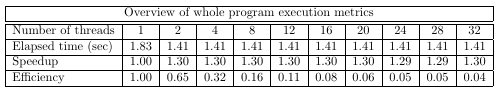
\includegraphics[width=0.9\linewidth]{fotosL4/primera_tabla_leaf.png}
    \caption{Model factor 1 (Leaf).}
    \label{fig:rec-leaf-mf1}
\end{figure}

\begin{figure}[H]
    \centering
    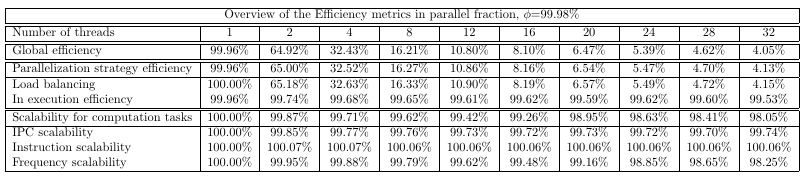
\includegraphics[width=0.9\linewidth]{fotosL4/segunda_tabla_leaf.png}
    \caption{Model factor 2 (Leaf).}
    \label{fig:rec-leaf-mf2}
\end{figure}

\begin{figure}[H]
    \centering
    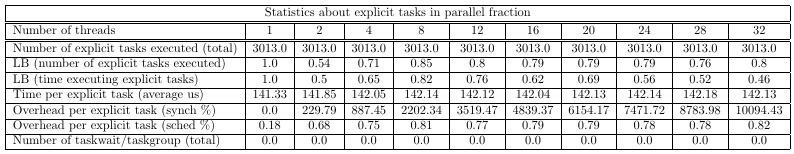
\includegraphics[width=0.9\linewidth]{fotosL4/tercera_tabla_leaf.png}
    \caption{Model factor 3 (Leaf).}
    \label{fig:rec-leaf-mf3}
\end{figure}
A la primera de les taules podem veure diversos aspectes que ens reflecteixen que no serà una implementació "molt bona". Veiem que l'Elapsed time, no baixa a partir de l'execució amb 2 threads amb un valor de 1.41 s, i que el Speedup no millora a partir de 2 threads, mantenint-se al voltant de 1.3. Això es veu reflectit en una eficiència molt baixa.\\
Això es deu a què el coll d'ampolla en aquest cas és la creació de tasques, que es fa de manera serial, i això provoca que la resta de threads estiguin inactius durant aquest procés. Per tant una execució amb 2 threads ja és suficient per mantenir ocupat el thread que crea les tasques i un altre que les executa, i afegir més threads no aporta cap millora.
Veiem a la taula 2 que el load balancing no es bo. Amb 2 threads és de 65\% i cau fins al 4.15\%, reduint-se a la meitar al duplicar el nombre de threads. Això es deu a la desigualtat en la creació de tasques, i a què hi ha tasques que tenen més cost que d'altres, els tiles de l'interior, i això provoca desequilibris.\\
De la tercera taula es destaca el nombre de tasques executades, que és 3013. Es compararà amb el nombre de tasques creat en altres apartats.

\subsection{Paraver Analysis}
\label{sec:rec-leaf-paraver}

% Paraver trace (useful/instantaneous parallelism and task creation view)
\begin{figure}[H]
    \centering
    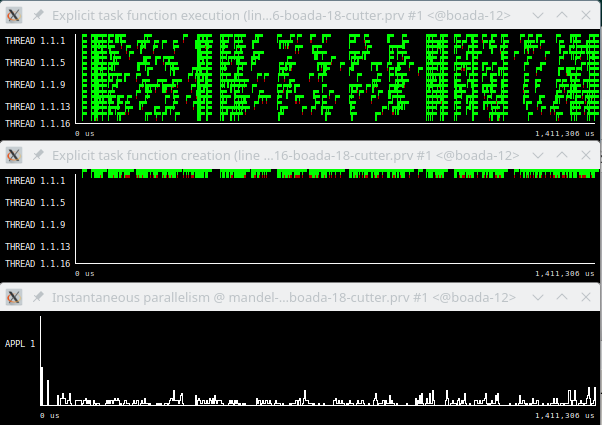
\includegraphics[width=0.9\linewidth]{fotosL4/paraver_leaf.png}
    \caption{Paraver trace for Recursive Leaf (16 threads): task creation and useful parallelism.}
    \label{fig:rec-leaf-paraver}
\end{figure}

A les traces obtingudes de Paraver, es pot observar, d'una banda, que la creació de tasques es fa únicament en un fil, i que la resta de fils es mantenen inactius fins que aquestes tasques es creen i s'assignen. Això es concorde amb l'anàlisi fet a la pràctica 3, on es va observar un desequilibri de càrrega entre la creació de tasques i la seva execució.
Podem veure però, que a l'hora de l'execució de les tasques, els 16 threads es mantenen actius, el que indica que la paralelització a nivell de tasques és efectiva un cop les tasques han estat creades.
A la tercera traça, es reflexa que el pararelisme és molt irregular, amb períodes de paralelisme útils seguits de períodes d'inactivitat. Això es deu a què, d'una banda a l'estratègia leaf no es creen totes les tasques a l'hora, i hi ha moments on no hi ha tasques disponibles per executar. D'altra banda, hi ha tasques que tenen més cost que d'altres, els tiles de l'interior, i això també provoca desequilibris.
Tot això reflexa la baixa eficiència del model de tasques en aquesta implementació, ja que 15 dels 16 threads estan inactius durant la creació de tasques i només es mantenen ocupats una vegada que les tasques han estat creades, i ho fan de manera irregular.

\subsection{Strong Scalability}
\label{sec:rec-leaf-scalability}

% Strong scalability plot
\begin{figure}[H]
    \centering
    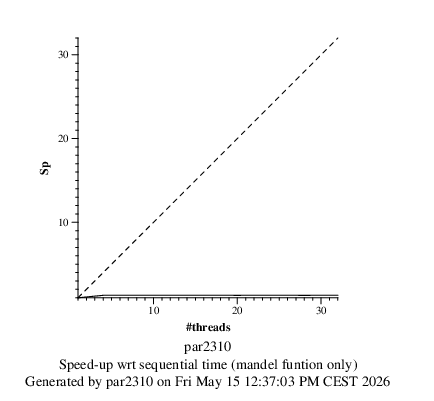
\includegraphics[width=0.75\linewidth]{fotosL4/grafico_leaf.png}
    \caption{Strong scalability (elapsed time vs. threads) for the Recursive Leaf implementation.}
    \label{fig:rec-leaf-speedup}
\end{figure}

De la figura prèvia en podem analitzar que l'increment de l'SpeedUp en relació al nombre de threads és nul, com ja haviem vist amb les taules modelfactor. Si que hi ha un increment de l'SpeedUp quan es passa de 1 a 2 threads, però a partir d'aquí no hi ha cap millora, mantenint-se al voltant de 1.3.\\
